%%% LaTeX Template
%%% This template is made for project reports
%%%	You may adjust it to your own needs/purposes
%%%
%%% Copyright: http://www.howtotex.com/
%%% Date: March 2011

%%% Preamble
\documentclass[paper=a4, fontsize=11pt]{scrartcl}	% Article class of KOMA-script with 11pt font and a4 format
\usepackage[T1]{fontenc}
\usepackage{fourier}

\usepackage[polutonikogreek, english]{babel}															% English language/hyphenation
\usepackage[iso-8859-7]{inputenc}
\usepackage[protrusion=true,expansion=true]{microtype}				% Better typography
\usepackage{amsmath,amsfonts,amsthm}										% Math packages
\usepackage[pdftex]{graphicx}														% Enable pdflatex
\usepackage{hyperref}
\usepackage{tabularx}
\usepackage{colortbl}
\usepackage{hhline}

%%% Custom sectioning (sectsty package)
\usepackage{sectsty}												% Custom sectioning (see below)
%\allsectionsfont{\centering \normalfont\scshape}	% Change font of al section commands
\sectionfont{\centering \normalfont\scshape}
\subsectionfont{\normalfont\scshape}


%%% Custom headers/footers (fancyhdr package)
\usepackage{fancyhdr}
\pagestyle{fancyplain}
\fancyhead{}														% No page header
\fancyfoot[C]{}													% Empty
\fancyfoot[R]{\thepage}									% Pagenumbering
\renewcommand{\headrulewidth}{0pt}			% Remove header underlines
\renewcommand{\footrulewidth}{0pt}				% Remove footer underlines
\setlength{\headheight}{13.6pt}


%%% Equation and float numbering
\numberwithin{equation}{section}		% Equationnumbering: section.eq#
\numberwithin{figure}{section}			% Figurenumbering: section.fig#
\numberwithin{table}{section}				% Tablenumbering: section.tab#


%%% Maketitle metadata
\newcommand{\horrule}[1]{\rule{\linewidth}{#1}} 	% Horizontal rule

\title{
		%\vspace{-1in} 	
		\usefont{OT1}{bch}{b}{n}
		\normalfont \normalsize \textsc{Automatic identification of kiwi calls from audio recordings} \\ [25pt]
		\horrule{0.5pt} \\[0.4cm]
		\huge Ornithokrites \\
		\horrule{2pt} \\[0.5cm]
}
\author{
		\normalfont 					\normalsize
        Lukasz Tracewski\\[-3pt]		\normalsize
        \today
}
\date{}


%%% Begin document
\begin{document}
\maketitle
\section{Overview}
Ornithokrites is a transliteration of ancient Greek {\selectlanguage{polutonikogreek}'orn"ijokr'iths}, meaning interpreter of flight or cries of birds. With its rather ambitious name, the program itself is a tool meant for an automatic identification of kiwi calls from low quality audio recordings. It has been designed to cope with large variations of environmental conditions and low quality of input data. For each provided audio file, the program enables detection of any kiwi calls and, in case they are present, which gender they belong to (male, female or both). \newline
Complete source code can be found on project's web site: \url{https://github.com/tracek/Ornithokrites}.

\section{How to use it}
Expected input are monaural (single-channel) audio files in Waveform Audio File Format (commonly known as WAV or WAVE). The following sections explain two ways of running the program: user-friendly \ref{sec:web_interface} and user-hostile \ref{sec:interactive_mode}.
\subsection{Web interface}
\label{sec:web_interface}
If the data is stored on Amazon Web Services S3 bucket, then by far the easiest way of using the program is through a password-protected web site: \url{http://kiwi-finder.info}. This protection is necessary since only one user at a time can run the program. \newline
After providing the credentials, the user is directed to a simple web form that serves as an interface to the application. The form contains the following:
\begin{itemize}
	\item Bucket name: name of Amazon Web Services S3 bucket, e.g. \textit{kiwicalldata}.
	\item E-mail address: if provided, an e-mail will be send to the given address once data processing is completed.
	\item Execute: connect to data store, download the recordings and run kiwi calls identification. It is a long-lasting operation. Closing the web page does not stop the program.
	\item Report: show results. Since they are generated live, user can click the button at any moment to get current state of affairs. Only text is printed, making it very fast.
	\item Show details: show detailed results. In this mode additional data is provided: spectrogram \ref{fig:spectrogram} with identified Regions Of Interest: blue triangles are detected male kiwi calls and green circles stand for female kiwi calls. Please keep in mind that a single detected kiwi call does not make a kiwi; only calls that appear in clusters are considered as candidates. Additionally, an option to play the original audio is provided, allowing the user to verify program's predictions.
	\item Clear: stop execution of the program and clear all intermediate results.
\end{itemize}

\begin{figure}[hbtp]
\label{fig:spectrogram}
\caption{Spectrogram of a recording after noise-reduction step showing male (blue triangles) and female (green circles) kiwi calls. }
\centering
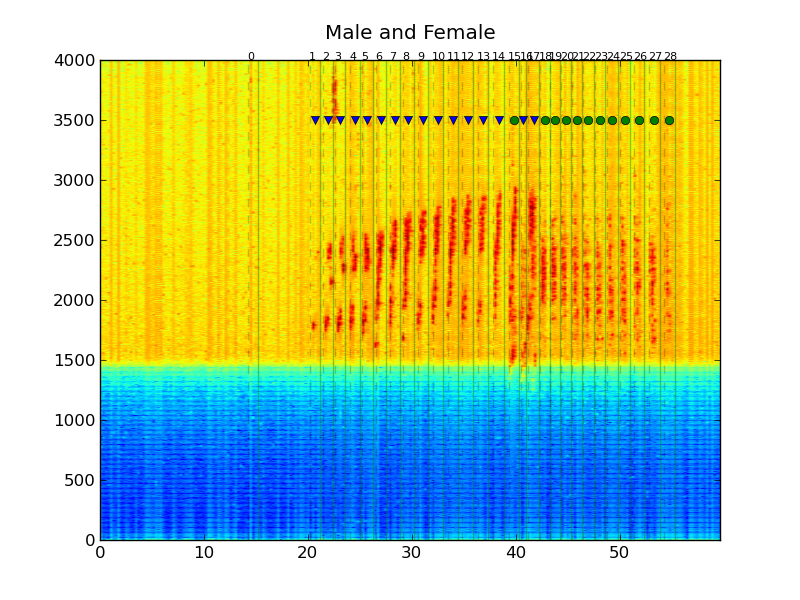
\includegraphics[scale=0.7]{spectrogram.png}
\end{figure}


\subsection{Interactive mode}
\label{sec:interactive_mode}
The program is written in Python, which means that running it directly (either from command line or in interactive mode) requires installation of all dependent modules. The complete list can be found on project's page. Due to the dependencies between modules, their installation may prove difficult.
\subsubsection{Batch mode - command line}
Executing program with '-h' switch, i.e. \texttt{ornithiokrites.py -h}, will print the complete help with command line arguments explained. This mode allows batch processing of files stored on a disc.
\subsubsection{Single-file mode - graphical user interface}
If no command line arguments are provided then program will start in interactive mode. With open file dialogue user can select a single file for analysis.
\section{How it works}
After the recordings are ready following steps take place:
\begin{enumerate}
	\item \textbf{Apply high-pass filter}. This step will reduce strength of any signal below 1500 Hz. Previous experiments have demonstrated that kiwi rarely show any vocalization below this value. It also helps to eliminate bird calls which are of no interest to the user, e.g. morepork.
	\item \textbf{Find Regions of Interest} (ROIs), defined as any signal different than background noise. Since length of a single kiwi call is roughly constant, ROI length is fixed to one second. First onsets are found by calculating local energy of the input spectral frame and taking those above certain dynamically-assessed threshold. Then from the detected onset a delay of $-0.2$s is taken to compensate for possible discontinuities. End of ROI is defined as $+0.8$s after beginning of the onset, summing to $1$s interval. The algorithm is made sensitive, since the potential cost of not including kiwi candidate in a set of ROIs is much higher then adding noise-only ROI.
	\item \textbf{Reduce noise}. Since ROIs are identified, Noise-Only Regions (NORs) can be estimated as anything outside ROIs (including some margin). Based on NORs spectral subtraction is performed: knowing noise spectrum we can try to eliminate noise over whole sample.
	\item \textbf{Calculate Audio Features}. Those features will serve as a kiwi audio signature, allowing to discriminate kiwi male from female - and a kiwi from any other animals. For each ROI following features are calculated:
	\begin{itemize}
		\item perceptual spread
		\item perceptual sharpness
		\item spectral flatness
		\item spectral roll-off
		\item spectral decrease
		\item spectral shape statistics
		\item spectral slope
		\item Linear Predictive Coding (LPC)
		\item Line Spectral Pairs (LSP)
		\item Octave Band Signal Intensity (OBSI)
	\end{itemize}
	Audio Features are calculated with \texttt{Yaafe} library. On its project page \url{http://yaafe.sourceforge.net/features.html} a complete description of above-mentioned features can be found.
	\item \textbf{Perform kiwi identification}. At this stage Audio Features are extracted from the recording. Based on these, a Machine Learning algorithm, that is Support Vector Machine (SVM), will try to classify ROI as kiwi male, kiwi female and not a kiwi. Additional rules are then applied, employing our knowledge on repetitive character of kiwi calls. Only in case a sufficiently long set of calls is identified, the kiwi presence is marked. 
	\item \textbf{Report}. Algorithm output can be: female, male, male and female and no kiwi detected.
\end{enumerate}

\section{Validation results}
Program was tested using stratified 5-fold cross-validation \footnote{\url{http://en.wikipedia.org/wiki/Cross-validation_\%28statistics\%29}}. Per Region Of Interest model got 93\% accuracy in distinguishing between a kiwi and "not a kiwi", and 90\% overall accuracy. Per file, those numbers raise to 99\% and 97\% respectively, which is possible due to employment of the most prominent feature of kiwi calls: their repetitive character. 

\begin{table}[hp]
\label{tab:confusion}
\caption{Confusion matrix}
\begin{tabularx}{.7\textwidth}{c|c c c c |}
 & Kiwi Male & Kiwi Female & Male and Female & \multicolumn{1}{c}{Not a kiwi} \\
\hhline{-----}
Kiwi Male & 65 \cellcolor[gray]{.8}& 0 & 0 & 1 \\
Kiwi Female & 0 & 35 \cellcolor[gray]{.8}& 0 & 0 \\
Male and Female & 1 & 3 & 26 \cellcolor[gray]{.8} & 0 \\
Not a kiwi & 0 & 0 & 0 & 30 \cellcolor[gray]{.8} \\
\hhline{~----}
\end{tabularx}
\end{table}

As visualised in the confusion matrix \footnote{\url{http://en.wikipedia.org/wiki/Confusion_matrix}} (table \ref{tab:confusion}), the program may misclassify a file when male and female are chatting label the pair as either Male or Female.

Since the program was trained on 1-minute samples, it very well might be that many times longer recordings will require a bit different approach with respect to noise reduction - and thus prove more challenging to the algorithm; nothing that cannot be fixed with more training data.

Processing of a single, one-minute file takes roughly 2 seconds on a single core of Intel Core-i5 @ 3.40 GHz. However, since the program features parallel computations, it can be made \textit{k}-times faster, where \textit{k} is the number of available cores. On the mentioned system with 4 cores processing of 206 files takes around 100 seconds.

\section{Developer's notes}
Following notes provide more technical information of little interest for the end user.
\subsection{Technology}
Ornithokrites is written in Python 2.7, with all of its heavy-duty numerical computations done in C/C++ compiled libraries. Comments in the code were formatted according to NumPy guidelines, ensuring they can be easily extracted by a capable program (e.g. Spyder). Program was tested on Linux, although, given enough determination, it should be also possible to run it on Windows and Mac OS.
\subsection{Machine Learning algorithm}
The Machine Learning algorithm used in this program, that is Support Vector Machine with Gaussian kernel, belongs to a class of supervised models. As a consequence, it requires labelled training set for fitting the model. At this moment 3318 fragments were classified as either male, female or not a kiwi. It is a manual task, with the labelling dependant on an individual proficiency in kiwi identification - and hence prone to errors.

\section{Acknowledgments}
I wish to thank Barry Polley from Department of Conservation of New Zealand for providing this utmost interesting challenge and his assistance along the way. My great appreciation also goes to Pat Miller of \url{birdingNZ.net} community that supplied me with invaluable help concerning kiwi identification; without his aid I would not be able to achieve such high accuracy.

\section{Contact information}
My e-mail: \href{mailto:lukasz.tracewski@gmail.com}{lukasz.tracewski@gmail.com}
\newline
Project's web page: \url{https://github.com/tracek/Ornithokrites}.

%%% End document
\end{document}
